\renewcommand\thesection{\arabic{section}}
\renewcommand\thesubsection{\thesection.\arabic{subsection}}



\textbf{Goal}:

This step aims to detect the wood knots on the target surface which will be segmented through the previews process. Ideal output will be shown in Figure~\ref{fig:mock2}.

\hspace*{\fill}

\textbf{Data set}:

An annotated data set of 640 images taken in a wood workshop in Schweinfurt and an unlabelled data set of 296 images from the historic roof construction of the Dominican church in Bamberg are available for the detection of wooden knots. Further datasets based on various historic timber structures are under consideration.

\hspace*{\fill}

\begin{figure}[ht]
  \centering
    \begin{subfigure}[b]{0.4\textwidth}
      \centering
        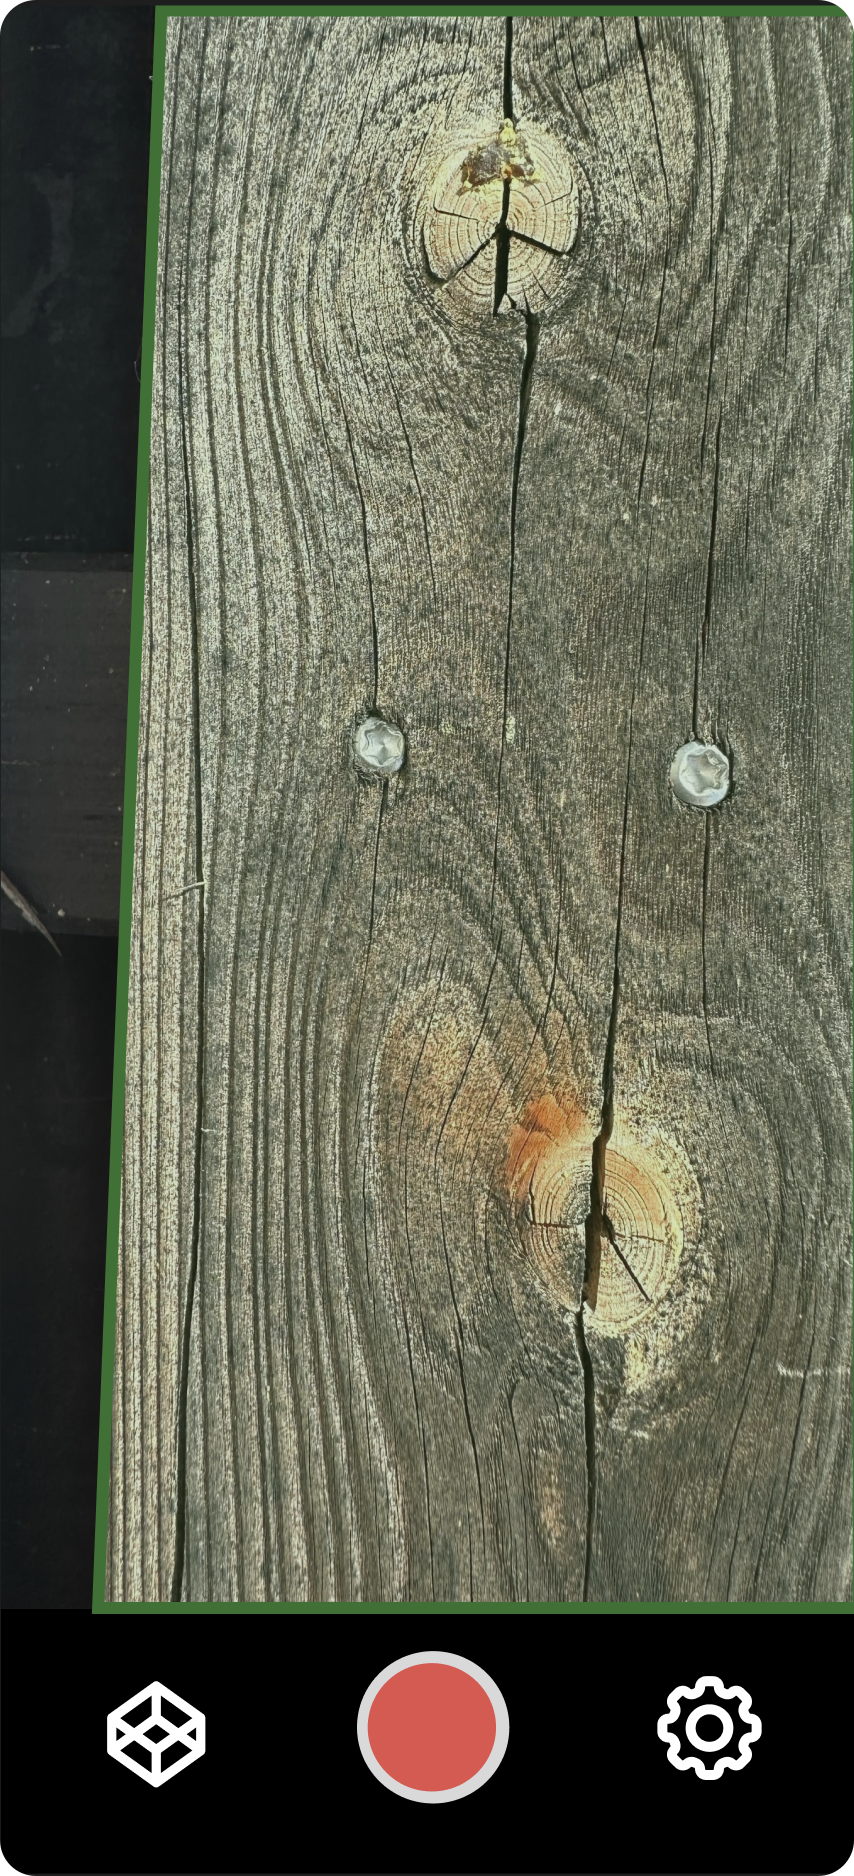
\includegraphics[width=0.55\textwidth]{Master Thesis/Images/Section_3/Mock/3-Mock2.png}
    \end{subfigure}
    \begin{subfigure}[b]{0.4\textwidth}
      \centering
        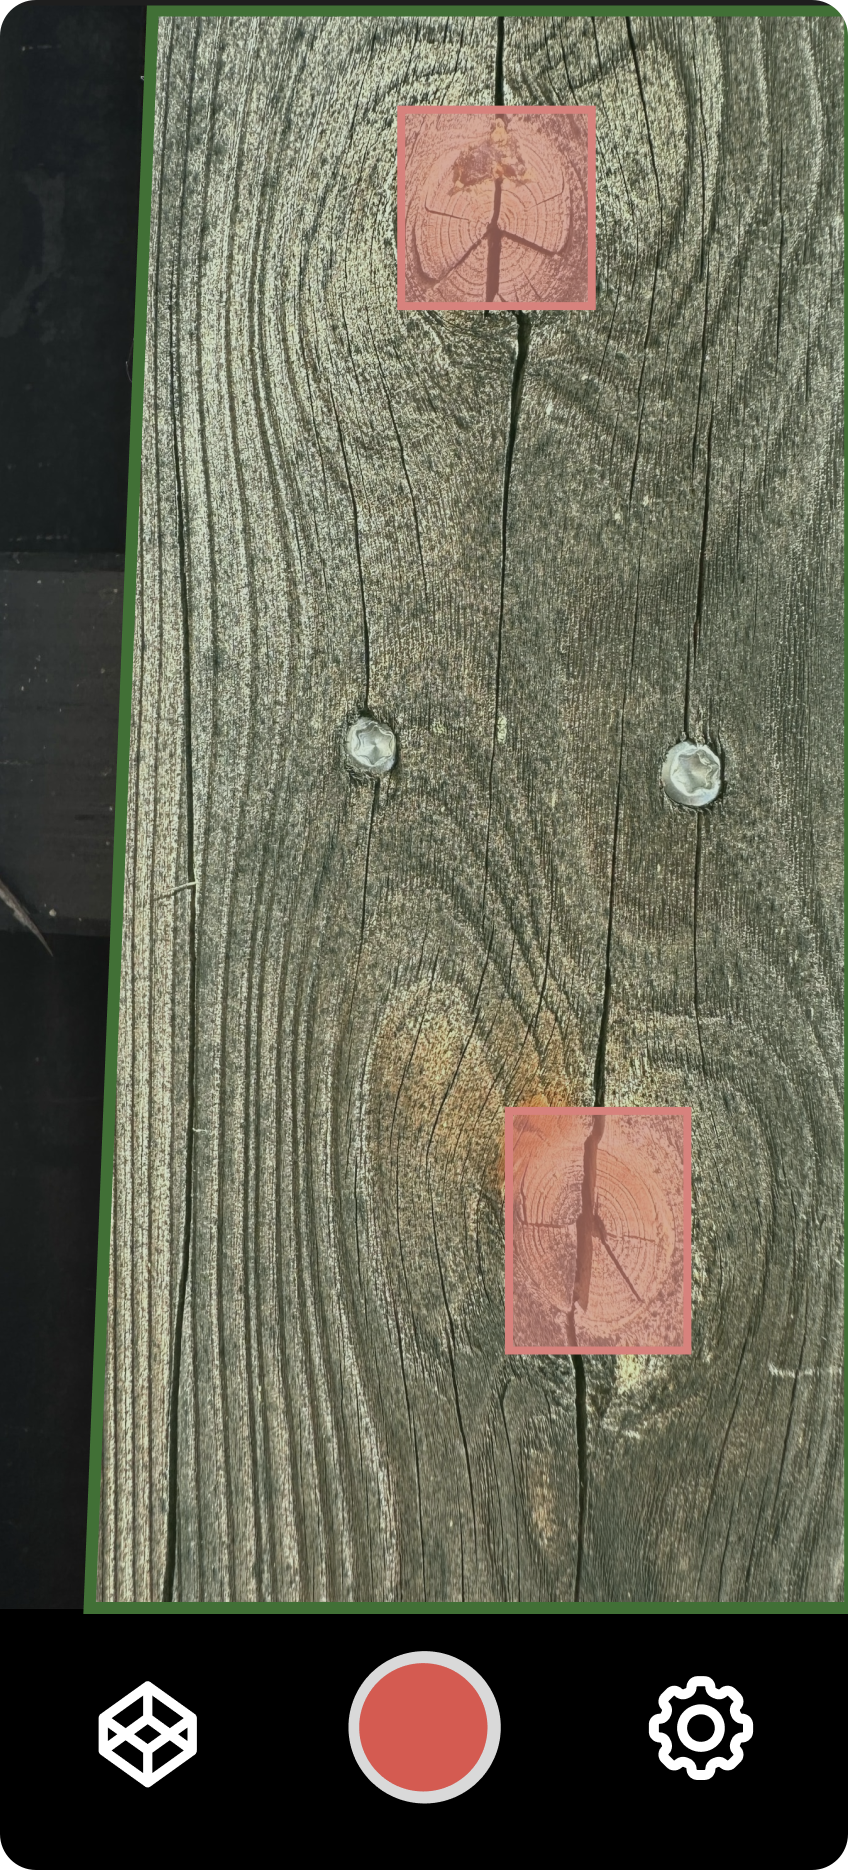
\includegraphics[width=0.55\textwidth]{Master Thesis/Images/Section_3/Mock/3-Mock3.png}
    \end{subfigure}
  \caption{Mocked-up output through detection of wooden knots}   
    \label{fig:mock2}
\end{figure}  

\textbf{Potential methods}:

In the earlier experiments, YOLOv8~\citep{yolov8_ultralytics} was used to test the performance of detection on wood knots using the mentioned self-captured dataset (Figure~\ref{fig:yolo_dataset}). The figure~\ref{fig:yolo_results} shows the results within the first experiments, which also show some insufficient bad cases that were wrongly detected. On the other hand, the SSD (single shot multibox detector, \citep{jia2014caffe}) also shows a potentially ideal performance. Both models should be further fine-tuned and optimised. 

\begin{figure}[htbp]
\centering
\begin{minipage}[t]{0.4\linewidth}
\centering
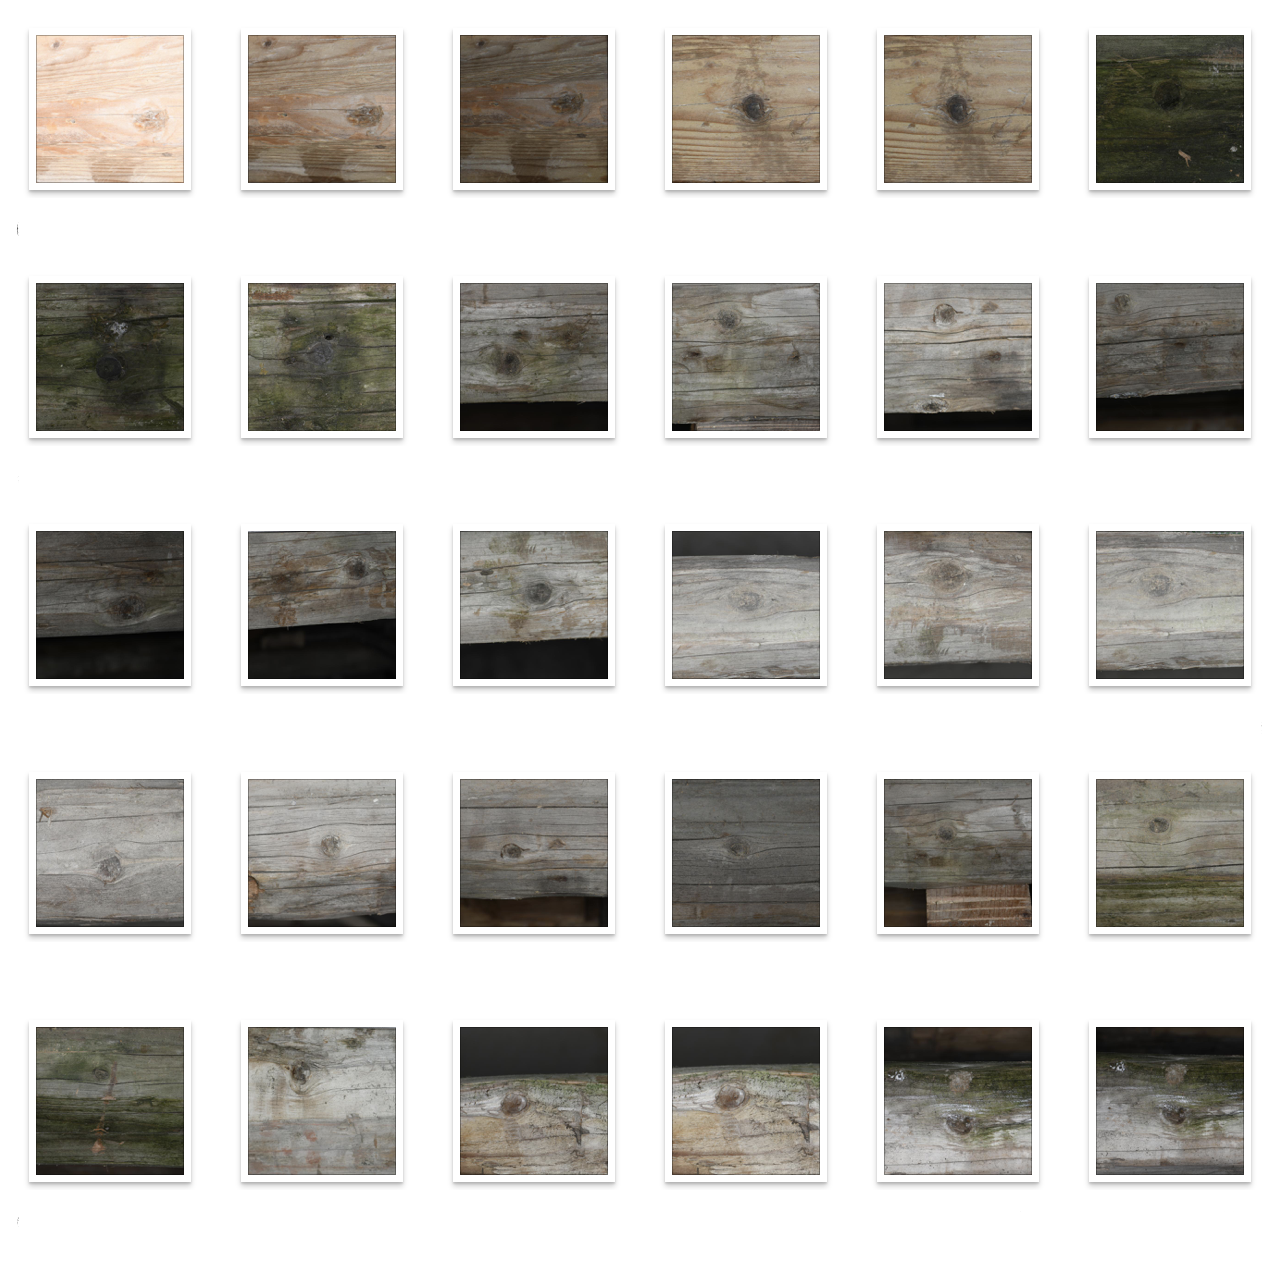
\includegraphics[height=4cm,width=4cm]{Master Thesis/Images/Section_3/Test_YOLO/3-dataset.png}
\caption{\parbox[t]{0.7\textwidth}{Annotated Data set with wood knots in bounding box}}
\label{fig:yolo_dataset}
\end{minipage}%
\hfill
\begin{minipage}[t]{0.6\linewidth}
\centering
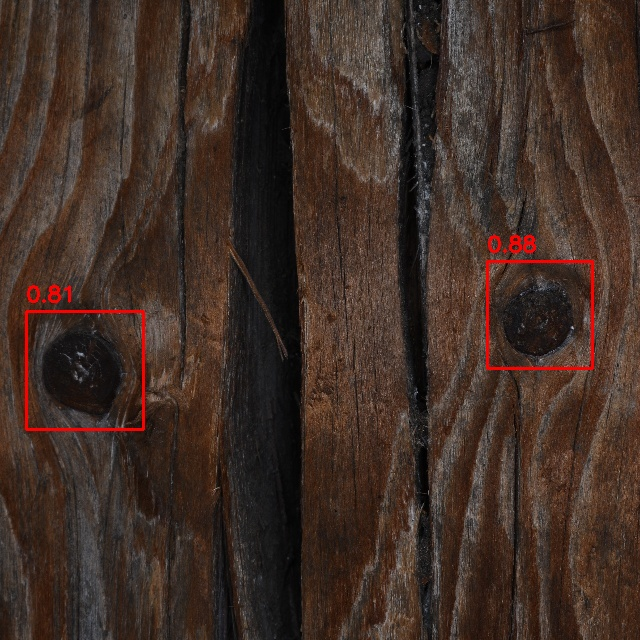
\includegraphics[height=4cm,width=4cm]{Master Thesis/Images/Section_3/Test_YOLO/3-007_3679_resize.JPG}
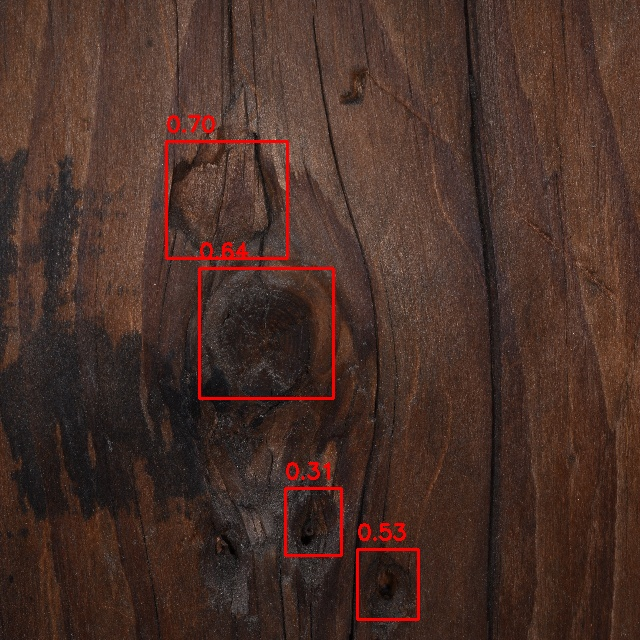
\includegraphics[height=4cm,width=4cm]{Master Thesis/Images/Section_3/Test_YOLO/3-007_3716_resize.JPG}
\caption{\parbox[t]{0.6\textwidth}{Results using YOLOv8m with 100 epochs}}
\label{fig:yolo_results}
\end{minipage}
\end{figure}

\hspace*{\fill}

\textbf{Output}:

The output is an image with the detected knots in bounding box and the position of the bounding box, which should be inside the detected area from previous segmentation process. (Figure~\ref{fig:mock2})


